% Created by tikzDevice version 0.10.1 on 2016-05-17 00:53:12
% !TEX encoding = UTF-8 Unicode
\documentclass{standalone}\usepackage{tikz}
\usepackage[utf8]{inputenc}
\usepackage[T1]{fontenc}
\usepackage[scaled]{helvet}
  \renewcommand{\familydefault}{\sfdefault}
%\usepackage[active,tightpage,psfixbb]{preview}

%\PreviewEnvironment{pgfpicture}

%\setlength\PreviewBorder{0pt}
\begin{document}

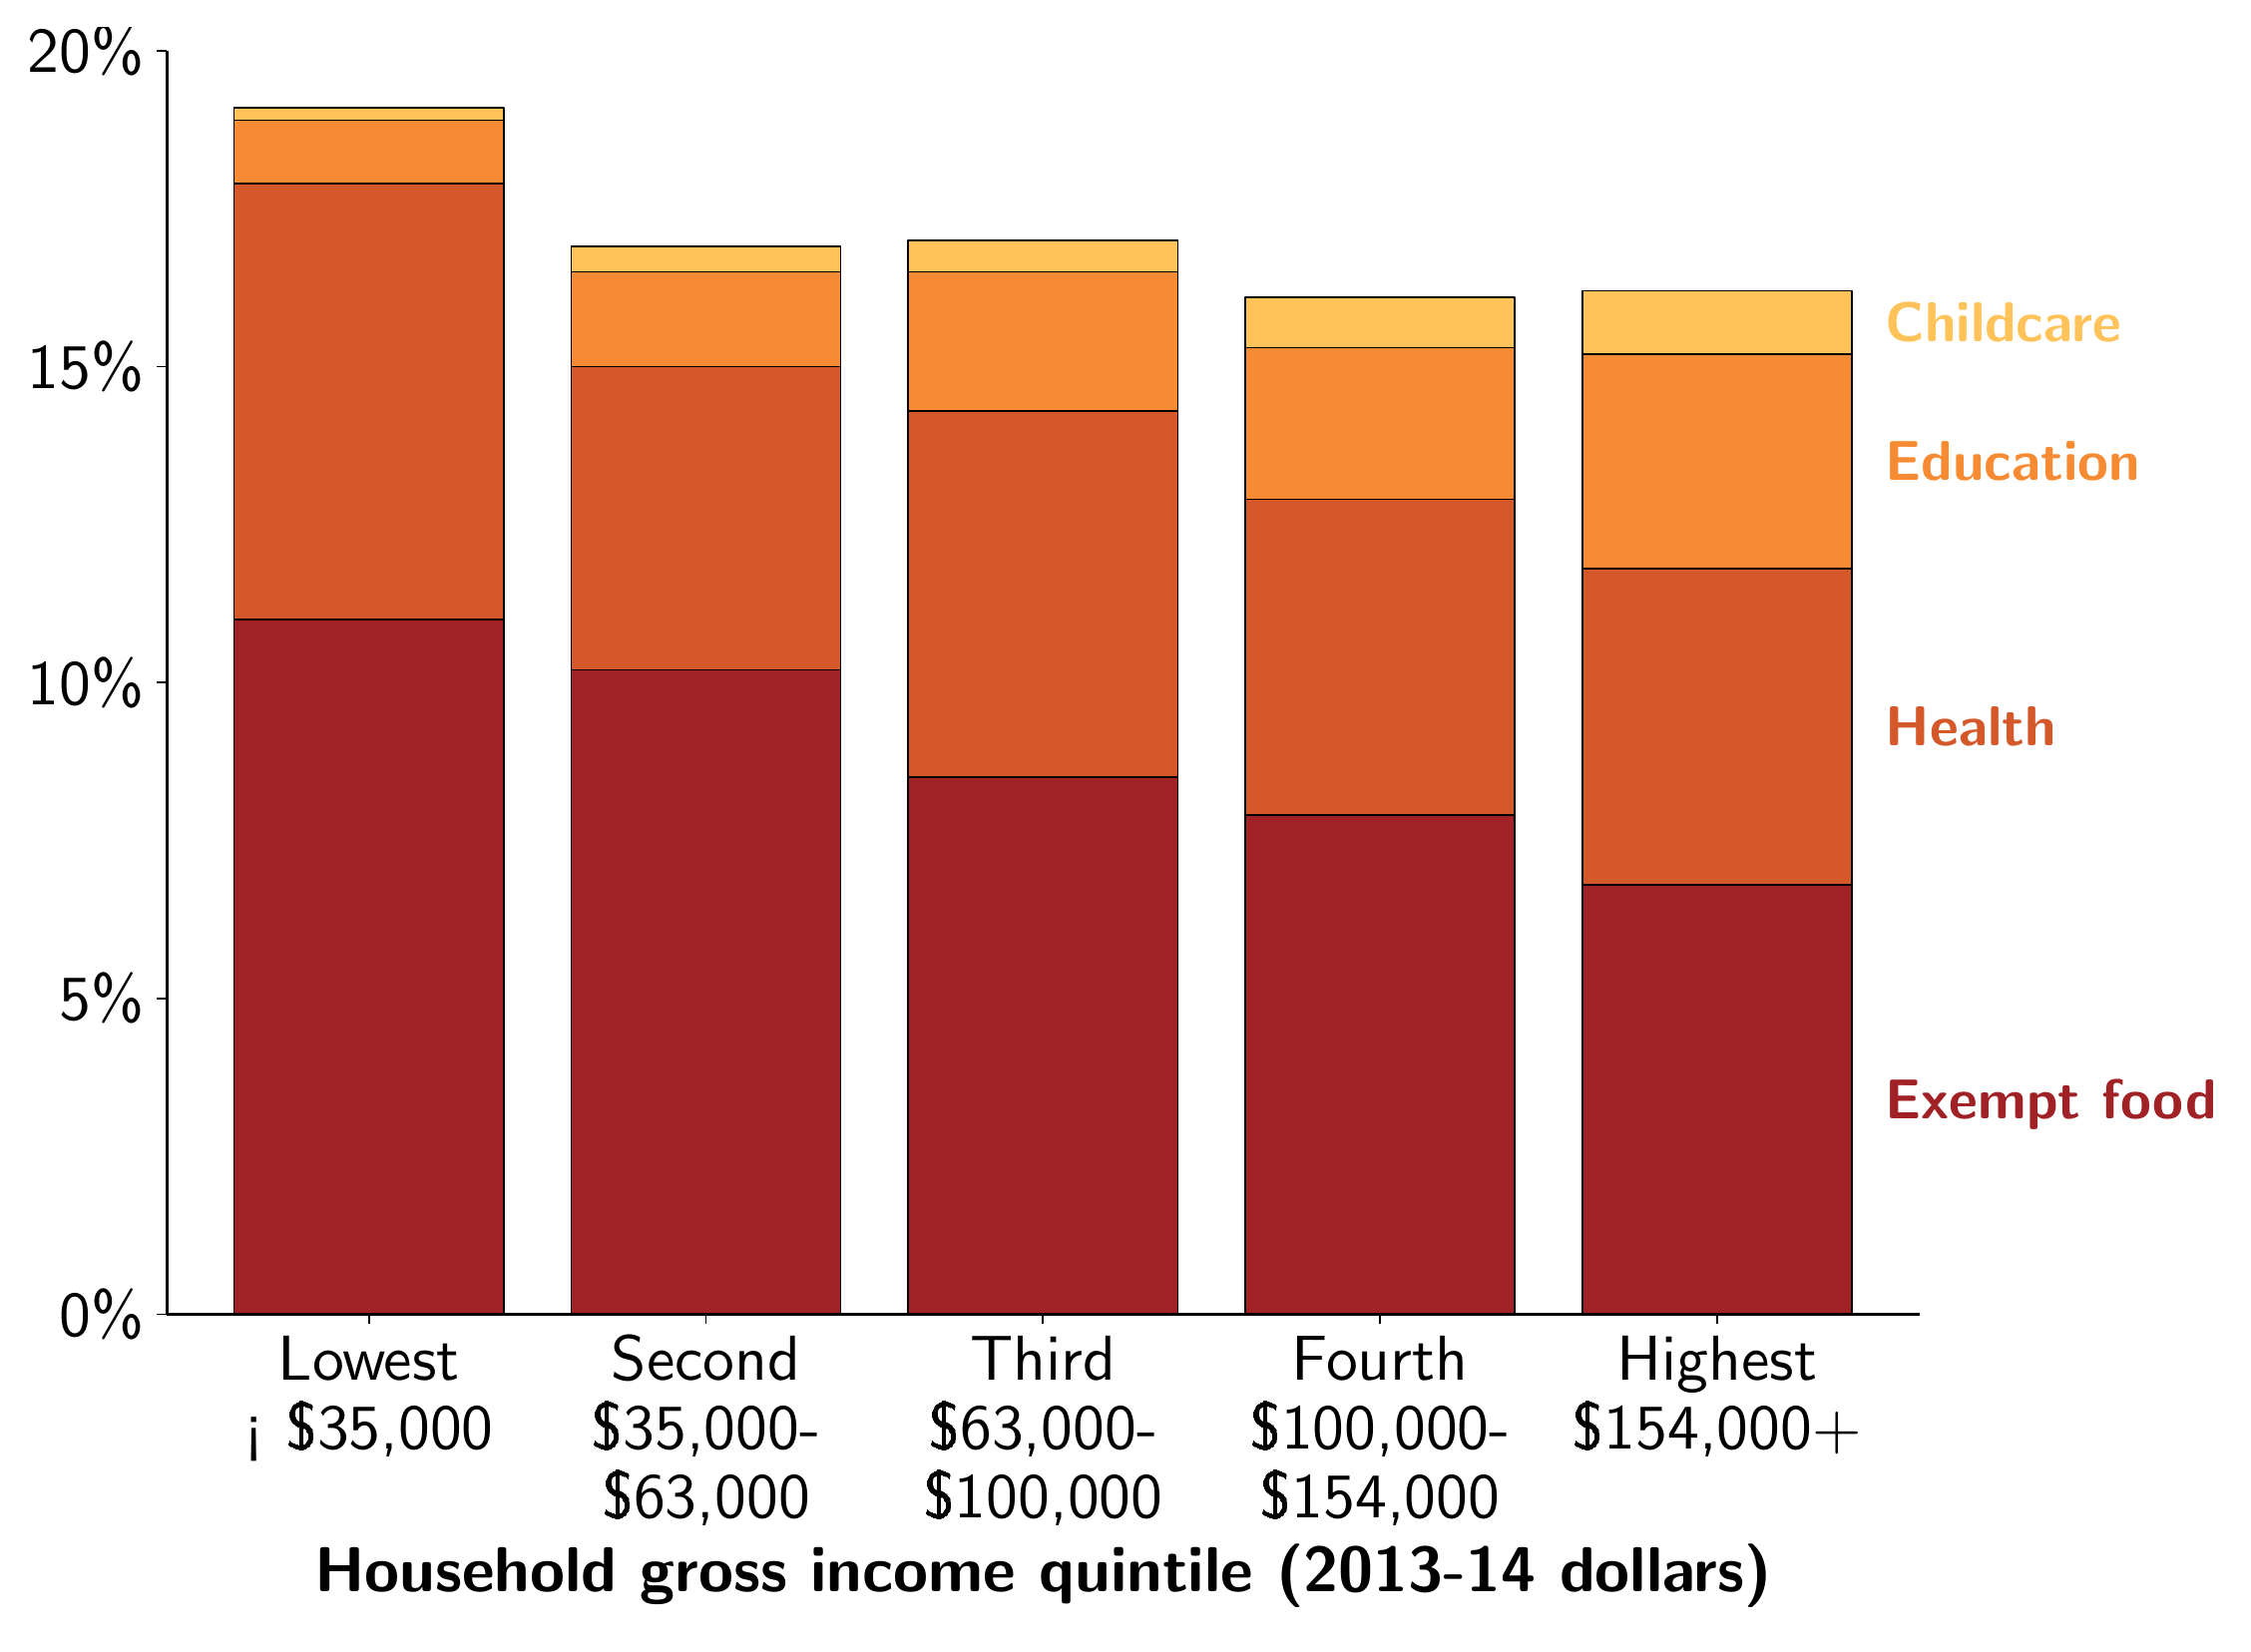
\begin{tikzpicture}[x=1pt,y=1pt]
\definecolor{fillColor}{RGB}{255,255,255}
\path[use as bounding box,fill=fillColor,fill opacity=0.00] (0,0) rectangle (794.97,578.16);
\begin{scope}
\path[clip] (  0.00,  0.00) rectangle (794.97,578.16);
\definecolor{drawColor}{RGB}{0,0,0}
\definecolor{fillColor}{RGB}{160,34,38}

\path[draw=drawColor,line width= 0.6pt,line join=round,fill=fillColor] ( 74.78,112.13) rectangle (172.43,363.81);
\definecolor{fillColor}{RGB}{212,88,42}

\path[draw=drawColor,line width= 0.6pt,line join=round,fill=fillColor] ( 74.78,363.81) rectangle (172.43,521.68);
\definecolor{fillColor}{RGB}{246,139,51}

\path[draw=drawColor,line width= 0.6pt,line join=round,fill=fillColor] ( 74.78,521.68) rectangle (172.43,544.56);
\definecolor{fillColor}{RGB}{255,195,90}

\path[draw=drawColor,line width= 0.6pt,line join=round,fill=fillColor] ( 74.78,544.56) rectangle (172.43,549.14);
\definecolor{fillColor}{RGB}{160,34,38}

\path[draw=drawColor,line width= 0.6pt,line join=round,fill=fillColor] (196.84,112.13) rectangle (294.48,345.50);
\definecolor{fillColor}{RGB}{212,88,42}

\path[draw=drawColor,line width= 0.6pt,line join=round,fill=fillColor] (196.84,345.50) rectangle (294.48,455.33);
\definecolor{fillColor}{RGB}{246,139,51}

\path[draw=drawColor,line width= 0.6pt,line join=round,fill=fillColor] (196.84,455.33) rectangle (294.48,489.65);
\definecolor{fillColor}{RGB}{255,195,90}

\path[draw=drawColor,line width= 0.6pt,line join=round,fill=fillColor] (196.84,489.65) rectangle (294.48,498.80);
\definecolor{fillColor}{RGB}{160,34,38}

\path[draw=drawColor,line width= 0.6pt,line join=round,fill=fillColor] (318.89,112.13) rectangle (416.54,306.61);
\definecolor{fillColor}{RGB}{212,88,42}

\path[draw=drawColor,line width= 0.6pt,line join=round,fill=fillColor] (318.89,306.61) rectangle (416.54,439.31);
\definecolor{fillColor}{RGB}{246,139,51}

\path[draw=drawColor,line width= 0.6pt,line join=round,fill=fillColor] (318.89,439.31) rectangle (416.54,489.65);
\definecolor{fillColor}{RGB}{255,195,90}

\path[draw=drawColor,line width= 0.6pt,line join=round,fill=fillColor] (318.89,489.65) rectangle (416.54,501.09);
\definecolor{fillColor}{RGB}{160,34,38}

\path[draw=drawColor,line width= 0.6pt,line join=round,fill=fillColor] (440.95,112.13) rectangle (538.59,292.88);
\definecolor{fillColor}{RGB}{212,88,42}

\path[draw=drawColor,line width= 0.6pt,line join=round,fill=fillColor] (440.95,292.88) rectangle (538.59,407.28);
\definecolor{fillColor}{RGB}{246,139,51}

\path[draw=drawColor,line width= 0.6pt,line join=round,fill=fillColor] (440.95,407.28) rectangle (538.59,462.19);
\definecolor{fillColor}{RGB}{255,195,90}

\path[draw=drawColor,line width= 0.6pt,line join=round,fill=fillColor] (440.95,462.19) rectangle (538.59,480.50);
\definecolor{fillColor}{RGB}{160,34,38}

\path[draw=drawColor,line width= 0.6pt,line join=round,fill=fillColor] (563.01,112.13) rectangle (660.65,267.71);
\definecolor{fillColor}{RGB}{212,88,42}

\path[draw=drawColor,line width= 0.6pt,line join=round,fill=fillColor] (563.01,267.71) rectangle (660.65,382.11);
\definecolor{fillColor}{RGB}{246,139,51}

\path[draw=drawColor,line width= 0.6pt,line join=round,fill=fillColor] (563.01,382.11) rectangle (660.65,459.90);
\definecolor{fillColor}{RGB}{255,195,90}

\path[draw=drawColor,line width= 0.6pt,line join=round,fill=fillColor] (563.01,459.90) rectangle (660.65,482.78);
\definecolor{drawColor}{RGB}{160,34,38}

\node[text=drawColor,anchor=base west,inner sep=0pt, outer sep=0pt, scale=  2.03] at (672.86,182.91) {\bfseries Exempt food};
\definecolor{drawColor}{RGB}{212,88,42}

\node[text=drawColor,anchor=base west,inner sep=0pt, outer sep=0pt, scale=  2.03] at (672.86,317.90) {\bfseries Health};
\definecolor{drawColor}{RGB}{246,139,51}

\node[text=drawColor,anchor=base west,inner sep=0pt, outer sep=0pt, scale=  2.03] at (672.86,414.00) {\bfseries Education};
\definecolor{drawColor}{RGB}{255,195,90}

\node[text=drawColor,anchor=base west,inner sep=0pt, outer sep=0pt, scale=  2.03] at (672.86,464.33) {\bfseries Childcare};
\end{scope}
\begin{scope}
\path[clip] (  0.00,  0.00) rectangle (794.97,578.16);
\definecolor{drawColor}{RGB}{0,0,0}

\path[draw=drawColor,line width= 1.1pt,line join=round] ( 50.37,112.13) --
	( 50.37,569.73);
\end{scope}
\begin{scope}
\path[clip] (  0.00,  0.00) rectangle (794.97,578.16);
\definecolor{drawColor}{RGB}{0,0,0}

\node[text=drawColor,anchor=base east,inner sep=0pt, outer sep=0pt, scale=  2.30] at ( 42.16,104.21) {0{\%}};

\node[text=drawColor,anchor=base east,inner sep=0pt, outer sep=0pt, scale=  2.30] at ( 42.16,218.61) {5{\%}};

\node[text=drawColor,anchor=base east,inner sep=0pt, outer sep=0pt, scale=  2.30] at ( 42.16,333.01) {10{\%}};

\node[text=drawColor,anchor=base east,inner sep=0pt, outer sep=0pt, scale=  2.30] at ( 42.16,447.41) {15{\%}};

\node[text=drawColor,anchor=base east,inner sep=0pt, outer sep=0pt, scale=  2.30] at ( 42.16,561.81) {20{\%}};
\end{scope}
\begin{scope}
\path[clip] (  0.00,  0.00) rectangle (794.97,578.16);
\definecolor{drawColor}{RGB}{0,0,0}

\path[draw=drawColor,line width= 0.6pt,line join=round] ( 46.76,112.13) --
	( 50.37,112.13);

\path[draw=drawColor,line width= 0.6pt,line join=round] ( 46.76,226.53) --
	( 50.37,226.53);

\path[draw=drawColor,line width= 0.6pt,line join=round] ( 46.76,340.93) --
	( 50.37,340.93);

\path[draw=drawColor,line width= 0.6pt,line join=round] ( 46.76,455.33) --
	( 50.37,455.33);

\path[draw=drawColor,line width= 0.6pt,line join=round] ( 46.76,569.73) --
	( 50.37,569.73);
\end{scope}
\begin{scope}
\path[clip] (  0.00,  0.00) rectangle (794.97,578.16);
\definecolor{drawColor}{RGB}{0,0,0}

\path[draw=drawColor,line width= 1.1pt,line join=round] ( 50.37,112.13) --
	(685.06,112.13);
\end{scope}
\begin{scope}
\path[clip] (  0.00,  0.00) rectangle (794.97,578.16);
\definecolor{drawColor}{RGB}{0,0,0}

\path[draw=drawColor,line width= 0.6pt,line join=round] (123.60,108.52) --
	(123.60,112.13);

\path[draw=drawColor,line width= 0.6pt,line join=round] (245.66,108.52) --
	(245.66,112.13);

\path[draw=drawColor,line width= 0.6pt,line join=round] (367.72,108.52) --
	(367.72,112.13);

\path[draw=drawColor,line width= 0.6pt,line join=round] (489.77,108.52) --
	(489.77,112.13);

\path[draw=drawColor,line width= 0.6pt,line join=round] (611.83,108.52) --
	(611.83,112.13);
\end{scope}
\begin{scope}
\path[clip] (  0.00,  0.00) rectangle (794.97,578.16);
\definecolor{drawColor}{RGB}{0,0,0}

\node[text=drawColor,anchor=base,inner sep=0pt, outer sep=0pt, scale=  2.30] at (123.60, 88.08) {Lowest};

\node[text=drawColor,anchor=base,inner sep=0pt, outer sep=0pt, scale=  2.30] at (123.60, 63.24) {< {\$}35,000};

\node[text=drawColor,anchor=base,inner sep=0pt, outer sep=0pt, scale=  2.30] at (245.66, 88.08) {Second};

\node[text=drawColor,anchor=base,inner sep=0pt, outer sep=0pt, scale=  2.30] at (245.66, 63.24) {{\$}35,000-};

\node[text=drawColor,anchor=base,inner sep=0pt, outer sep=0pt, scale=  2.30] at (245.66, 38.40) {{\$}63,000};

\node[text=drawColor,anchor=base,inner sep=0pt, outer sep=0pt, scale=  2.30] at (367.72, 88.08) {Third};

\node[text=drawColor,anchor=base,inner sep=0pt, outer sep=0pt, scale=  2.30] at (367.72, 63.24) {{\$}63,000-};

\node[text=drawColor,anchor=base,inner sep=0pt, outer sep=0pt, scale=  2.30] at (367.72, 38.40) {{\$}100,000};

\node[text=drawColor,anchor=base,inner sep=0pt, outer sep=0pt, scale=  2.30] at (489.77, 88.08) {Fourth};

\node[text=drawColor,anchor=base,inner sep=0pt, outer sep=0pt, scale=  2.30] at (489.77, 63.24) {{\$}100,000-};

\node[text=drawColor,anchor=base,inner sep=0pt, outer sep=0pt, scale=  2.30] at (489.77, 38.40) {{\$}154,000};

\node[text=drawColor,anchor=base,inner sep=0pt, outer sep=0pt, scale=  2.30] at (611.83, 88.08) {Highest};

\node[text=drawColor,anchor=base,inner sep=0pt, outer sep=0pt, scale=  2.30] at (611.83, 63.24) {{\$}154,000+};
\end{scope}
\begin{scope}
\path[clip] (  0.00,  0.00) rectangle (794.97,578.16);
\definecolor{drawColor}{RGB}{0,0,0}

\node[text=drawColor,anchor=base,inner sep=0pt, outer sep=0pt, scale=  2.30] at (367.72, 11.52) {\bfseries Household gross income quintile (2013-14 dollars)};
\end{scope}
\end{tikzpicture}

\end{document}
